\chapter{Link Analysis} 
Corresponding Text: \href{http://infolab.stanford.edu/~ullman/mmds/ch5.pdf}{Chapter 5 of MMDS}

\section{PageRank}
\subsection{Transition Matrix} 
Transition matrix is a column stochastic matrix. Entry $M_{ij}$ indicates the probability of going to $i$ from $j$. The long term limiting distribution is $v$ such that $v = Mv$ as long as two conditions are met: 
    \begin{itemize}
        \item The graph is strongly connected. It is possible to get from any node to any other node 
        \item There are no dead end
    \end{itemize}
    
\subsection{General Structure of the Web} 
A web in general are composed of 
    \begin{itemize}
        \item Strongly Connected Component (SCC) 
        \item The in-component: pages that could reach SCC but not reachable from SCC
        \item The out-component: pages that are reachable from SCC but can't reach SCC
        \item Tendrils: 1) pages reachable from the in-component, but not able to reach the in-component. 2) pages that can reach out-component, but not reachable from the out-component. 
        \item Tubes: pages reachable from the in-component and able to reach the out-component, but unable to reach the SCC or be reached from SCC
        \item Isolated component. 
    \end{itemize}
    
\subsection{Avoding dead-end and Spider Traps} 
PageRank needs to avoid two situations: 
    \begin{itemize}
        \item dead-end 
        \item spider traps: a group of pages that all have outlinks but they never link to any other pages 
    \end{itemize}
They can be solved via 
    \begin{itemize}
        \item Iteratively drop until no dead-end (after solving, nodes that got removed have their PageRank computed by summing over all predecessors PageRank divided by the number of successor of predecessor). 
        \item Taxation (randomly teleport to another page). $v' = \beta M v + (1 - \beta) \frac{e}{n}$. 
    \end{itemize}
    
\subsection{Efficient Computation of PageRank} 

\subsubsection{Representing Transition Matrices}
Transition matrix column can be represented by 
    \begin{itemize}
        \item one integer: out degree 
        \item one integer per nonzero entry in that column: the row numbers
    \end{itemize}

\subsubsection{Traditional Computation} 
One iteration of PageRank is $v' = \beta M v + (1 - \beta) \frac{e}{n}$. If $v$ can fit into main memory, then this is just a Matrix vector multiplication in Map Reduce. Otherwise, we can use the stripping technique discussed in the intro section. 

\subsection{Use Combiners to Consolidate the Result Vector} 
In certain circumstances we wish to add terms for $v_i'$, the $i-th$ entry of the $Mv$. However, that term most likely is not available in main memory because: 
    \begin{itemize}
        \item In the stripping technique, any vertical strip of $M$ + horizontal strip of $v$ will contribute to all components of the result vector $v'$
        \item $M$ is stored column-by-column. But one column can affect any of the component of $v'$
    \end{itemize}

Alternatively, we can partition the matrix into $k^2$ blocks while the vectors are still partitioned into $k$ strips. E.g.: Let $M = 4 \times 4$ and let $k=2$. The blocks of $M$ are $M_{11}, M_{12}, M_{21}, M_{22}$
    \begin{align*}
        \begin{bmatrix}
            \begin{bmatrix}
                m_{11} & m_{12} \\
                m_{21} & m_{22}
            \end{bmatrix}
            &
            \begin{bmatrix}
                m_{13} & m_{14} \\
                m_{23} & m_{24}
            \end{bmatrix}
            \\
            \begin{bmatrix}
                m_{31} & m_{32} \\
                m_{41} & m_{42}
            \end{bmatrix}
            & 
            \begin{bmatrix}
                m_{33} & m_{34} \\
                m_{43} & m_{44}
            \end{bmatrix}             
        \end{bmatrix}
        * 
        \begin{bmatrix}
            \begin{bmatrix}
                    v_1 \\ v_2
            \end{bmatrix}
            \\
            \begin{bmatrix}
                    v_3 \\ v_4
            \end{bmatrix}
        \end{bmatrix}
         = 
         \begin{bmatrix}
             \begin{bmatrix}
                M_{11} v_1 + M_{12}v_2       
             \end{bmatrix}
             \\
            \begin{bmatrix}
                M_{21} v_1 + M_{22}v_2       
             \end{bmatrix}
         \end{bmatrix}
    \end{align*}
Now, using $k^2$ Map tasks, each task gets one square of the matrix $M$, and one strip of the vector $v$. Notice that all the terms generated from $M_{ij}$ and $v_j$ contribute to $v'_i$ and no other stripes of $v'$ 

For each block, we need to store 
    \begin{itemize}
        \item columns that have at least one non-zero entry 
        \item list those rows that have a nonzero entry 
        \item outdegree for the column
    \end{itemize}
    
\subsection{Biased Random Walk} 
Only teleport to a subset of pages
\begin{align*}
    v' = \beta M v + (1 - \beta) \frac{e_s}{|S|}
\end{align*}


\section{Link Spam}
A spam farm can be constructed by pointing accessible pages to the target page and set up assisting pages for the target pages. The architecture is figure \ref{fig:spam_farm}. 
\begin{figure}[h]
    \centering
    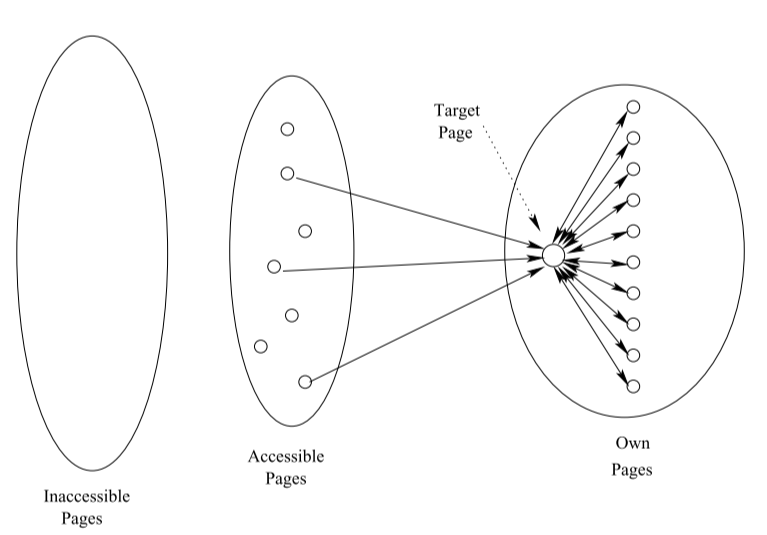
\includegraphics[height = 7cm, width = 8cm]{figs/004_spam_farm.PNG}
    \caption{Spam Farm Architecture}
    \label{fig:spam_farm}
\end{figure}
Let there be $n$ pages on the web in total. Let $t$ be the target page, and have $m$ supporting pages. Let $x$ be the amount of PageRank contributed by the accessible page. Let $y$ be the PageRank of the target page. The PageRank of each supporting page is 
    \begin{align*}
        \beta \frac{y}{m} + \frac{1 - \beta}{n}
    \end{align*}
The PageRank $y$ of target $t$ have 1) Contribution $x$ from outside, 2) $\beta$ times the PR of eary supporting page, 3) $(1-\beta)/n$ from taxation. 3 is normally so small that it doesn't matter. Combining 1 and 2 and solve for $y$ we get 
    \begin{align*}
        y = \frac{x}{1-\beta^2} + \frac{\beta}{1+\beta}\frac{m}{n}
    \end{align*}
If $\beta = 0.85$, we can see that $y$ now gets $\frac{1}{1-0.85^2}$ times boost to the original true contribution $x$, in addition to bonus PageRank determined by the fraction $\frac{m}{n}$. 

Two ways to combat SpamFarm is 
    \begin{itemize}
        \item TrustRank: Use a trust worthy (human examination / trust worthy domain) teleport set. 
        \item Spam Mass: $p = \frac{r-t}{r}$ where $t$ is the trust rank and $r$ is the page rank. If spam mass is close to 1 or high, eliminate the pages. 
    \end{itemize}
    
\section{Hubs and Authorities} 
Each web page has two scores: 
    \begin{itemize}
        \item $h$: hubbiness of a page (how many good content this page links to). 
        \item $a$: authority of a page (the quality of the content of this page) 
    \end{itemize}
The link matrix is an $n\times n$ matrix where $L_{ij}=1$ if there is a link from page $i$ to page $j$. The computation process is 
    \begin{enumerate}
        \item Initiate $h = 1$
        \item Compute $a = L^T h$, and scale so the largest component is $1$
        \item Compute $h = La$, scale so the largest component is $1$
        \item Repeat last two steps. 
    \end{enumerate}